\documentclass[12pt]{article}
\usepackage[utf8]{inputenc}
\usepackage{sectsty}
\usepackage{float, graphicx}
\graphicspath{ {./images/} }
\usepackage[margin=1.4in]{geometry}
\usepackage{multirow}
\usepackage{fancyhdr}
\pagestyle{fancy}
\renewcommand{\headrulewidth}{0pt}
\renewcommand{\footrulewidth}{1pt}
\begin{titlepage}
    \begin{center}
        \vspace*{1cm}
            
        \Huge
        \textbf{ Tank Water Level Meter (Group-18)}
            
        \vspace{1cm}
        \LARGE
        {An IoT device for monitoring water level}
        \vspace{1.5cm}
        \begin{figure}[H]
\centering
    
\includegraphics[scale=0.35]{NSUT_logo.png}
   
\end{figure}
        
            
        \vspace{1cm}
       
      \normalsize
      \begin{flushright}
              \textbf{Submitted To:\\}Prof. D.V.Gadre\vspace*{0.15cm}\\
              \textbf{Submitted By:\\\vspace*{0.15cm}}Arsh Kohli-2020UEC2509  \vspace{0.15cm}\\ Priyanshu-2020UEC2502\\\vspace*{0.15cm} Gurkirat Singh-2020UEC2552\vspace{0.45cm}\\
              Electronics Design and Workshop(EDW) Project\\ Netaji Subhas University of Technology\\ ECE-2024
      \end{flushright}
       
            
    \end{center}
\end{titlepage}

% \sectionfont{\fontsize{12}{18}\selectfont}
\begin{document}

\vspace{4cm}
\section*{Acknowledgement}
We would like to thank a few people without whom this project would certainly not have been possible. Gadre sir for his constant support and guidance. Thank you for sparking our interest in building something real, we had a ton of fun while putting this project together and are grateful for the hands-on approach that you took while teaching this course. Naman Puri bhaiyya for always being there to help us with anything related to our project. Thank you for patiently solving even the silliest doubts that we had. Rohan Deswal bhaiyya for helping us with the 3D printing process.
\vspace{20cm}

\section*{Synopsis}
\normalsize
We regularly come across a situation where we see an overflowing water tank, and often hear this colloquial phrase, \emph{“motor band kardo paani bhar gaya”}. So, we decided to develop a Tank Water Level System using components like  NodeMCU ESP8266 and an ultrasonic sensor- \emph{HC-SR04} with a primary aim to activate a buzzer whenever water tank is full. In addtion to that real time status of the tank is sent to the user using a WebApp, also it would provide the data regarding total water consumption of a household and would detect any kind of leakage in the tank. 
\section*{Motivation}
\normalsize
Our motive behind making this project is primarily to reduce wastage of water due to overflowing and leakages and also to calculate the daily water consumption. Although there are several other products in the market but they are not cost effective. So, we decided to make a very cost effective and efficient tank water meter.
\section*{Project Description}
\normalsize
\begin{itemize}
 \item Ultrasonic sensor-\emph{HC-SR04}
  \vspace{0.025cm}
  
  It is a sensor that can measure distance using echolocation. It emits ultrasound at 40 000 Hz (40kHz). A pulse is transmitted from the sensor and distance-to-water-level is determined by measuring the time required for the echo return from the water surface.

\begin{figure}[H]
\centering
    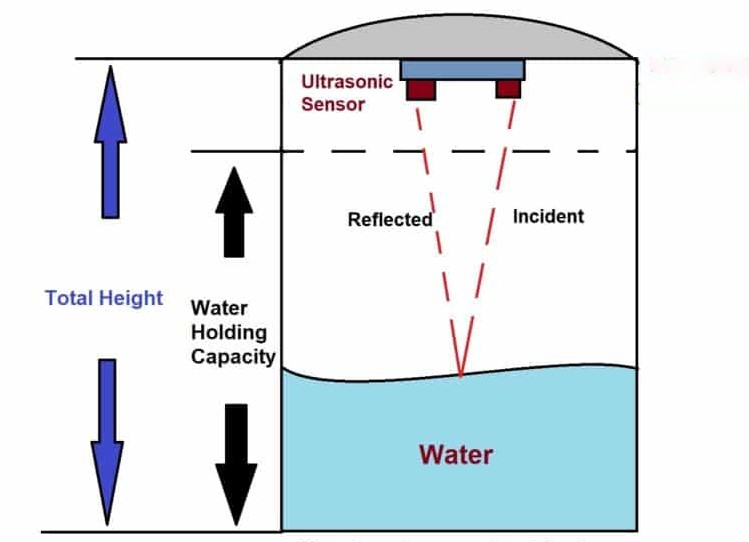
\includegraphics[scale=0.35]{ULtrasonic_sensor.jpg}
    \caption{Working of Ultrasonic sensor}
    \label{fig:my_label}
\end{figure}


\item NodeMCU ESP8266
    \vspace{0.025cm}
    
  The brain behind our whole project, NodeMCU ESP8266 is one type of microcontroller board, designed by Espressif Systems. It is a small size board which is  also flexible with a wide variety of applications. It performs all the functions ranging from calculating the tank size to sending information/status about the tank to the web app in real time. It has the capability to connect to WiFi inbuilt. Some technical specifications of the board are as follows:
  \vspace{0.025cm}
  
            Microcontroller: Tensilica 32-bit RISC CPU Xtensa LX106\\
            Operating voltage: 3.3 volts\\
            Input voltage: 7-12 volts\\
            Digital I/O pins: 16\\
             Analog input pins: 1\\
             Flash memory: 4 MB\\
             SRAM: 64 KB\\
              Clock speed: 80 MHz\\
\begin{figure}[H]
\centering
    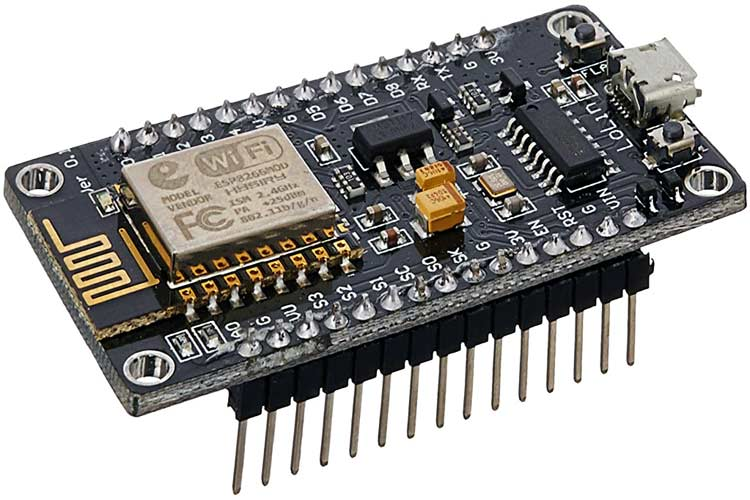
\includegraphics[scale=0.27]{node.jpg}
    \caption{ESP8266 NodeMCU}
    \label{fig:my_label}
\end{figure}


  \clearpage
  
\item Buzzer
\vspace{0.025cm}

 It is mainly used to prompt an alarm signal whenever water level goes above a certain threshold.

 \begin{figure}[H]
\centering
    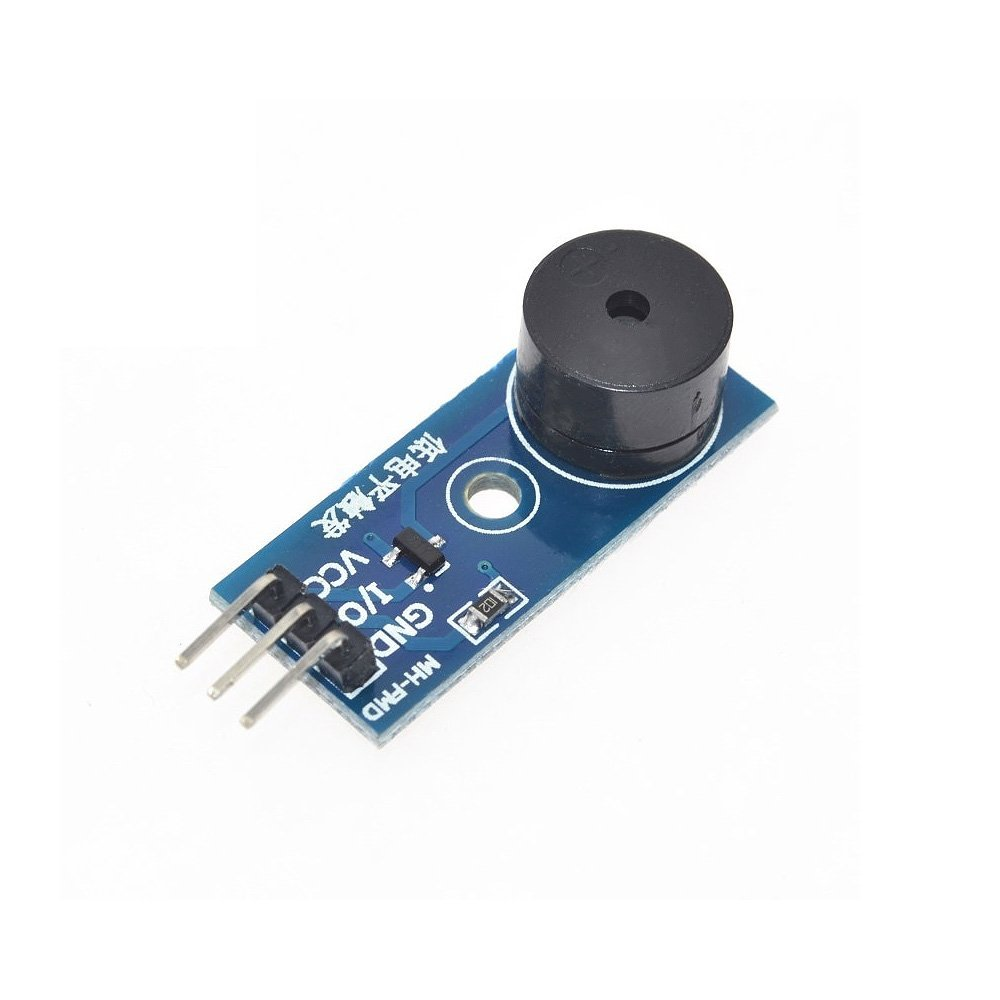
\includegraphics[scale=0.18]{buzzer.jpg}
    \caption{Buzzer}
    \label{fig:my_label}
\end{figure}
  \end{itemize}
\section*{Block Diagrams}
\normalsize
 \begin{figure}[H]
\centering
    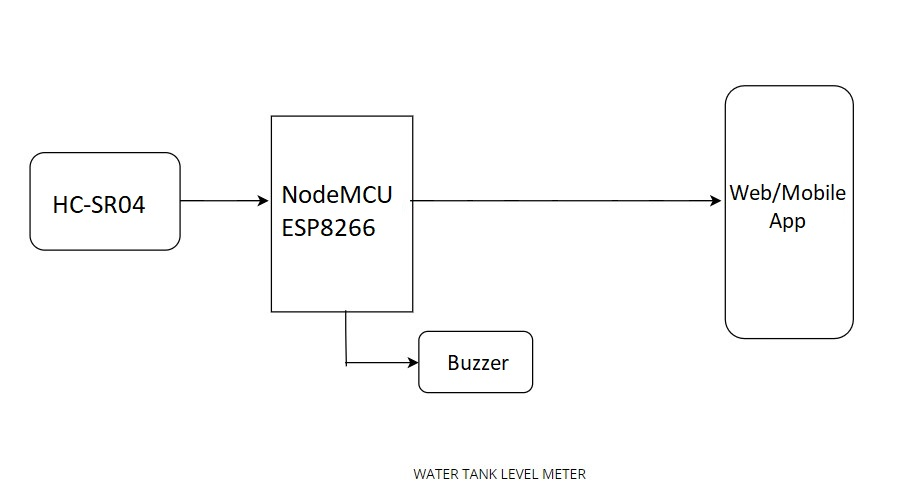
\includegraphics[scale=0.75]{bdiagram.jpg}
    \caption{Block diagram}
    \label{fig:my_label}
\end{figure}
\clearpage
\section*{Flowcharts}
\vspace{0.3cm}
 \begin{figure}[H]
\centering
    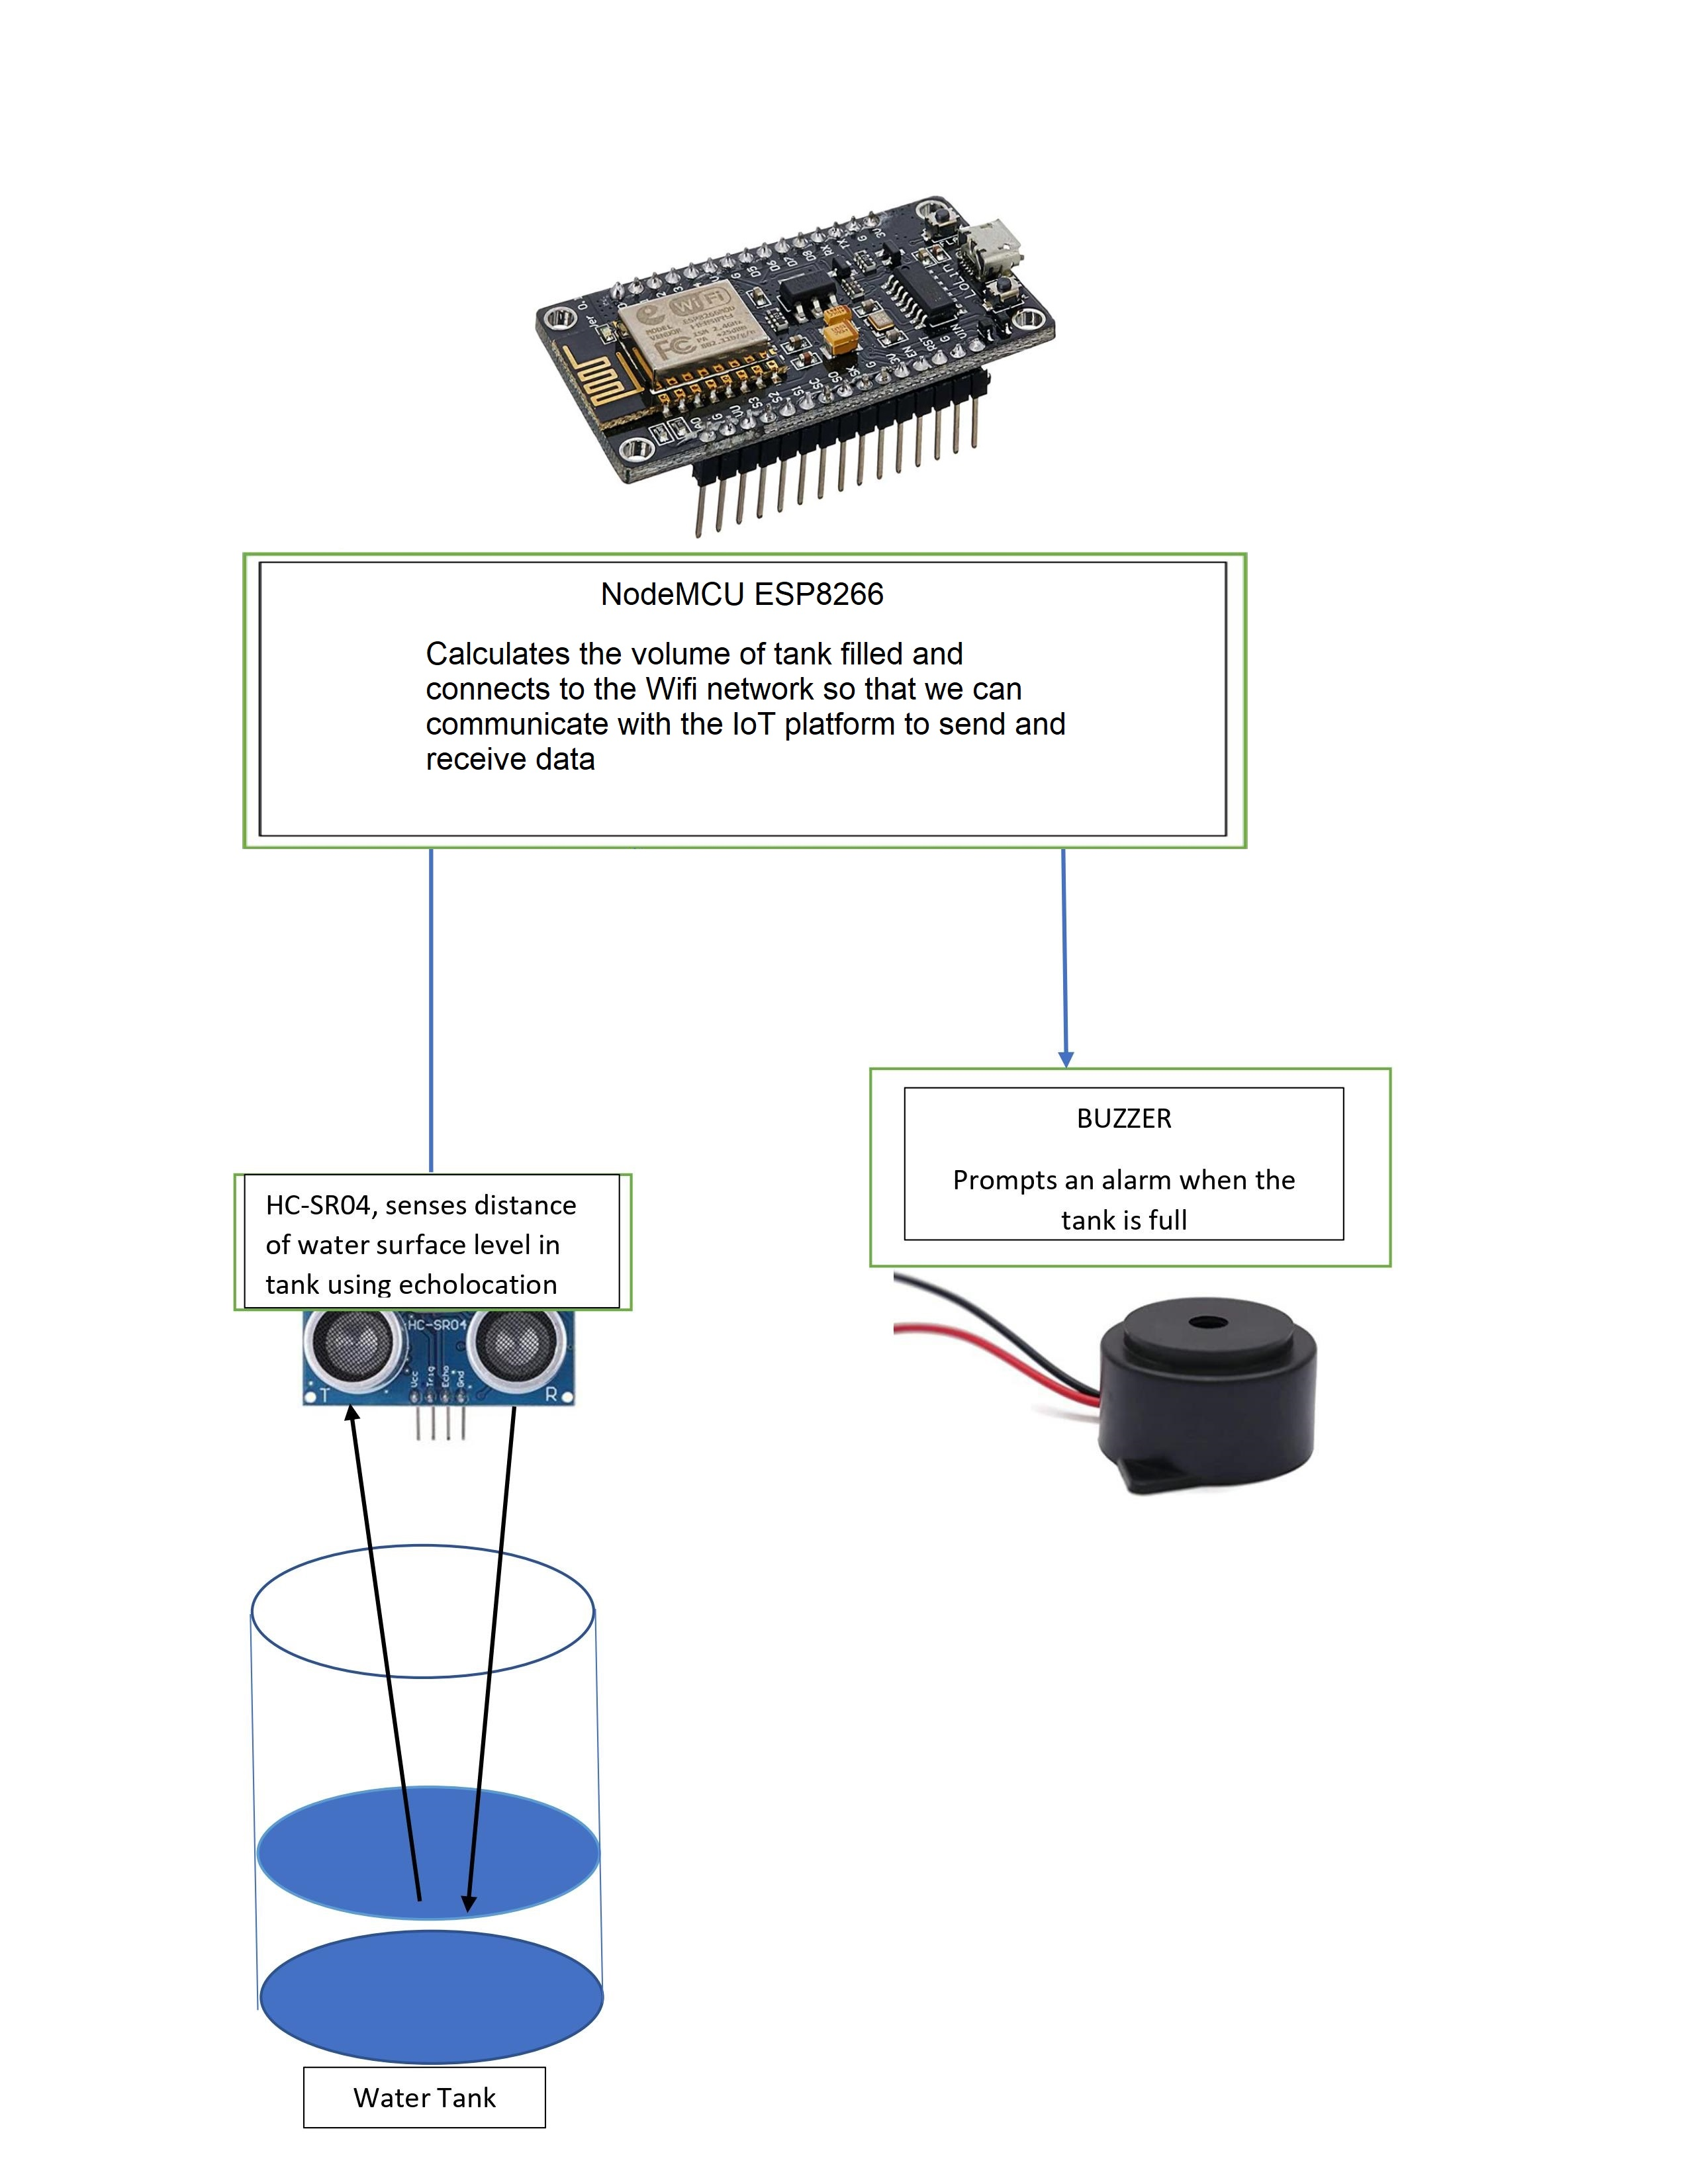
\includegraphics[scale=0.65]{01.jpg}
    \caption{Flow chart-1}
    \label{fig:my_label}
\end{figure}
\clearpage
\section*{Bill Of Materials}
\vspace{0.75cm}


\begin{tabular}{ |p{1cm}||p{7cm}|p{2cm}|p{2cm}|  }

 \hline
 
 \hline
 S.No & Component Name  &Quantity & Price\\
 \hline
 1 & NodeMCU ESP8266 & 1& 300-600\\
 2&	HC-SR406 ULTRASONIC SENSOR& 1&	110\\
 3&	BUZZER&	1&	50\\
 4&	ENCLOSING CASE&	1&	200-500\\
 5&	MISCELLANEOUS&	-&	400\\

 \hline
\end{tabular}
\vspace{0.3cm}
\section*{Gantt Chart}
 \begin{figure}[H]
    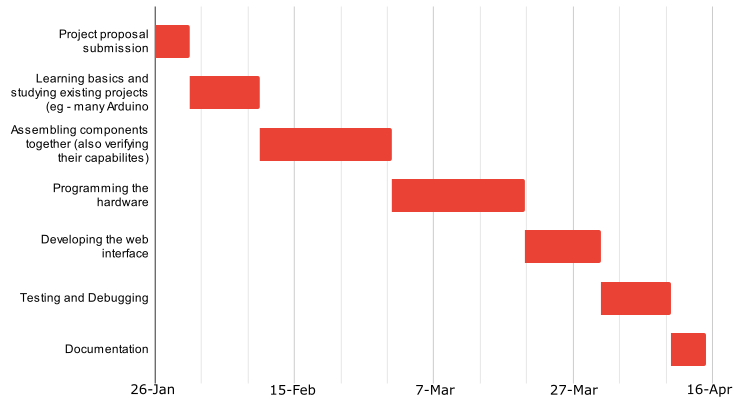
\includegraphics[scale=0.84]{Gantt4.png}
    \caption{Gantt Chart}
    \label{fig:my_label}
\end{figure}

\vspace{3cm}
\section*{Difficulties faced}
 \normalsize
\begin{itemize}
\item Programming the ESP8266 - We had initially started with an Arduino Nano as our main microcontroller. We had planned to use it to operate the ESP8266 module however after a bit of tinkering, we found out that the ESP8266 module cannot be operated by another microcontroller, it can only be programmed to operate a certain way such that its code is separated from the code that runs on the Arduino. This way, the Arduino essentially became an inefficient UART bridge that is used to program the ESP8266 chip. We solved this problem by switching to a NodeMCU ESP8266 (aka ESP-12) microcontroller.
\begin{figure}[H]
\centering
    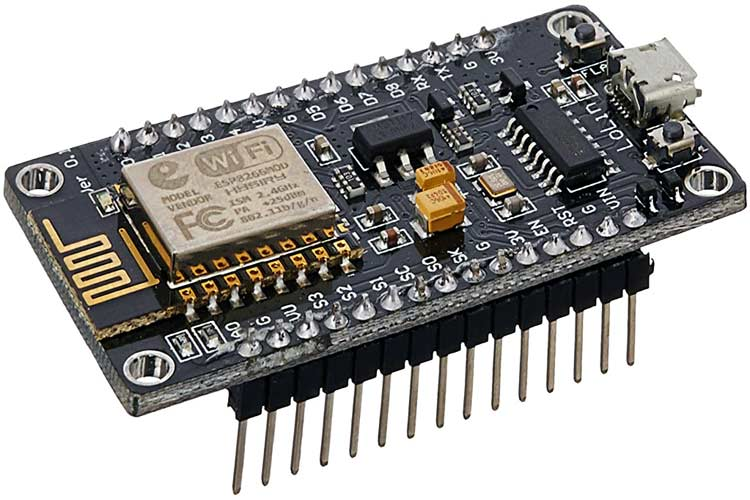
\includegraphics[scale=0.22]{node.jpg}
    \caption{ESP8266 NodeMCU}
\end{figure}
\item Power Issues - With the arduino, we often ran into issues where the ESP8266 module would randomly start outputting gibberish to the Serial Monitor. After hours of scouring through dozens of forums online, we figured out that the problem arose due to power issues. The Arduino could not supply enough power to the ESP8266 module, This was also solved when we switched to the NodeMCU ESP8266 microcontroller.
\begin{figure}[H]
\centering
    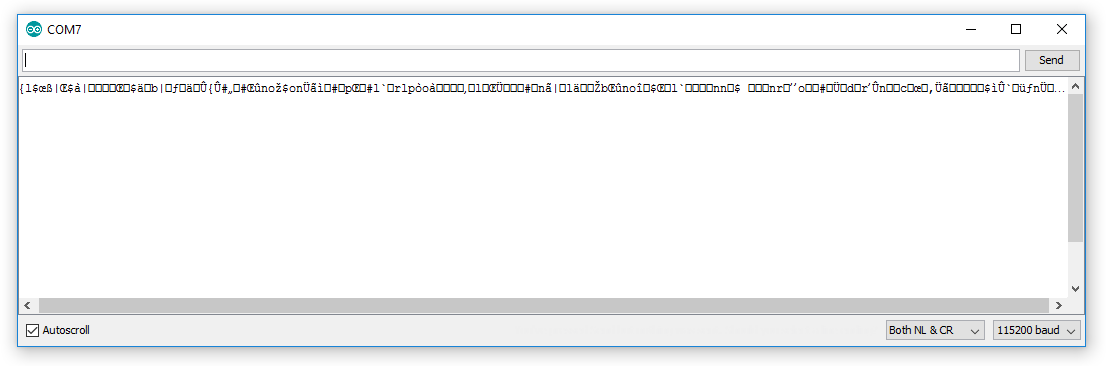
\includegraphics[scale=0.45]{serialgibb.png}
    \caption{Gibberish on the Serial Monitor}
\end{figure}
\item Driver Issues - The microcontroller would not respond to Serial AT (ATtention) commands in the beginning. After installing the relevant drivers and experimenting with different baud rates, we got it working.
\begin{figure}[H]
\centering
    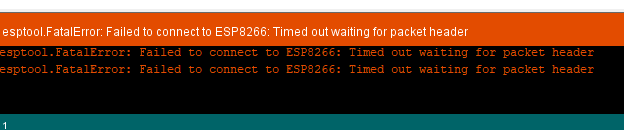
\includegraphics[scale=0.55]{timeout.png}
    \caption{Driver Issues while uploading the sketch}
\end{figure}
\item Complexities on the software side - Our plan initially was to send HTTP requests through the microcontroller and use it to trigger actions on the server side using an IoT service such as IFTTT or Thingspeak. The problem with these platforms was two-fold. First, they did not store past data which made plotting water level on a chart impossible without using another service (and increasing complexity). Secondly, they used HTTP to talk to the microcontroller which was inefficient. After some reasearch, we found a platform (Blynk) that kept logs of data and had a convenient library which abstracted the MQTT protocol for the ESP8266. The code had to be rewritten to use it instead of HTTP requests.
\begin{figure}[H]
\centering
    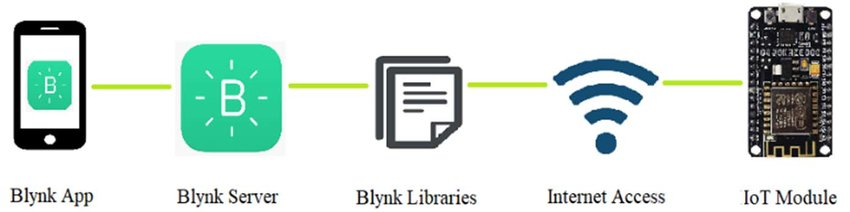
\includegraphics[scale=0.45]{blynk.jpg}
    \caption{Block diagram of our IoT stack}
\end{figure}
\end{itemize}

\vspace{8cm}

\section*{Code Explanation}
\begin{itemize}
\item On the software side of things, we are using Blynk, an IoT platform that makes it easier to integrate IoT devices with the cloud. Blynk has both a web interface and a mobile dashboard to monitor our devices outputs. We've set the outputs as virtual pins on the Blynk platform and our microcontroller (NodeMCU ESP8266) utilizes these to receive and send data to the Blynk server using the MQTT protocol.
\item The setup function runs at startup and sets the Ultrasonic sensor's trigger pin as output and its echo pin as input. The buzzer is set as an output pin. Then, it attempts to connect to our Wifi network.
\begin{figure}[H]
\centering
    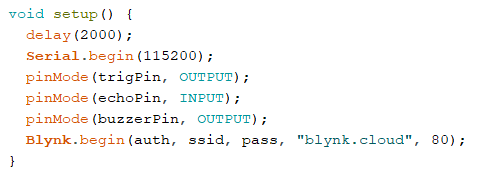
\includegraphics[scale=0.85]{setup.png}
    \caption{Setup function which runs on startup}
\end{figure}
\item The loop function first initiates a handshake to the Blynk server. In order to refresh the water level every 4 seconds, we keep checking if 4000 milliseconds have elapsed since the last time we checked and run the code under the if statement if the condition is satisfied. This delay period change be adjusted and is in the variable named timerDelay.
\item Next, we trigger an ultrasonic wave by setting the trigger pin of the Ultrasonic sensor to HIGH for a very short period of time (10 milliseconds). Now, we record the time before this wave returns to the Ultrasonic sensor. When it returns, after hitting the water level, our echo pin is set to HIGH. This time is recorded in a variable named "duration."
\begin{figure}[H]
\centering
    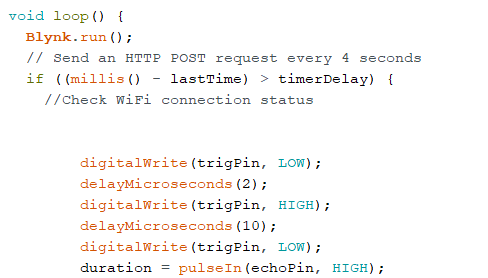
\includegraphics[scale=0.85]{loop1.png}
    \caption{First part of the loop function}
\end{figure}
\item Now, we calculate the distance of the water surface using the duration. Since we have the distance of the water surface when there is no water in the tank (in a variable name minLevel), we can use this to calculate the percentage of water filled in the tank. We trigger the buzzer if the tank is more than 50\% filled and buzzer alerts are turned on. After this, we update the percentage level through a virtual pin so we can track it on the Blynk platform's mobile app.
\begin{figure}[H]
\centering
    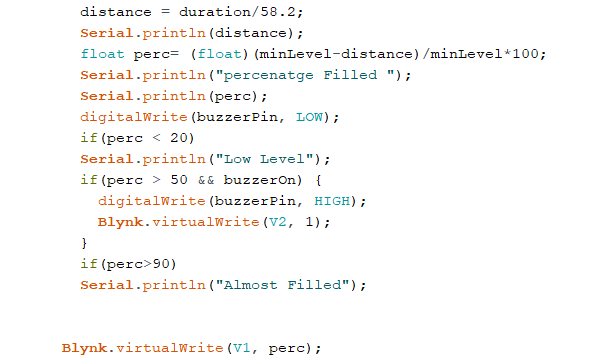
\includegraphics[scale=0.85]{loop2.png}
    \caption{Second part of the loop function}
\end{figure}
\end{itemize}
\section*{Gallery}
\begin{figure}[H]
\centering
    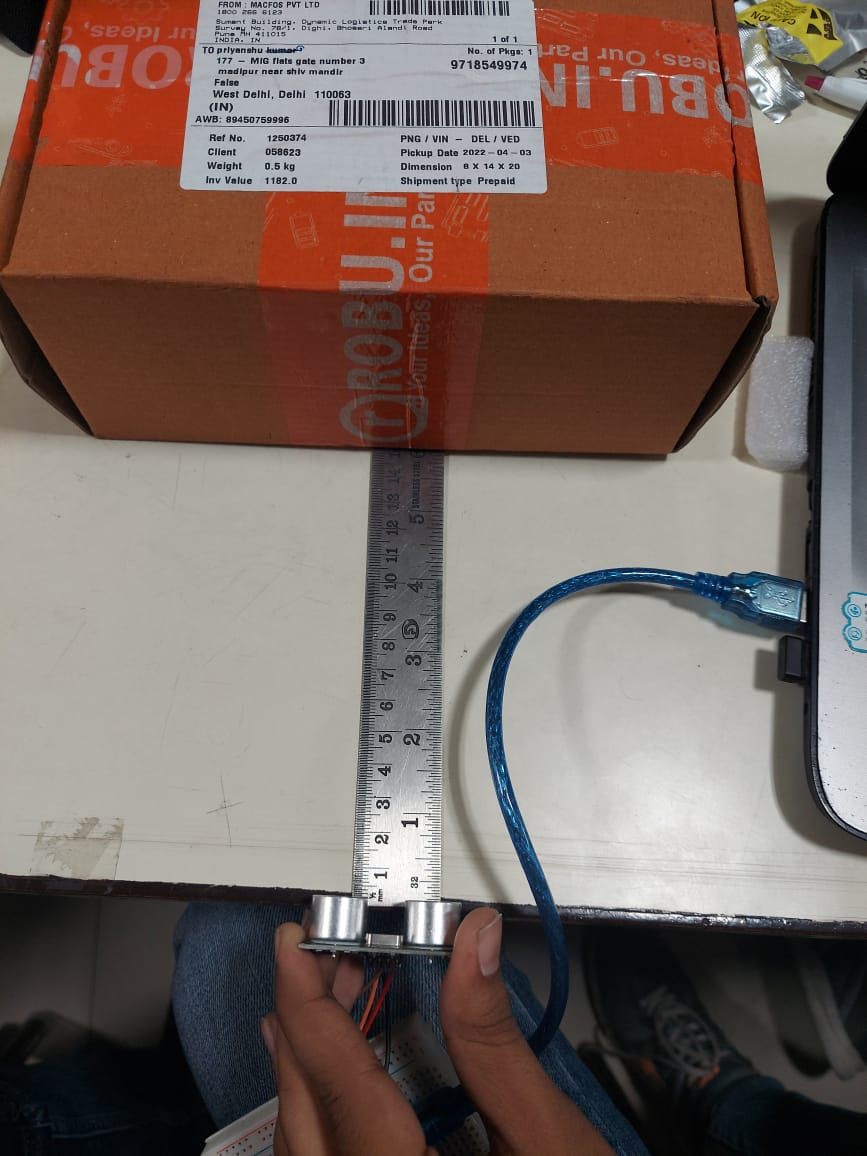
\includegraphics[scale=0.20]{ultra1.jpg}
    \caption{Testing Ultrasonic sensor}
\end{figure}
\begin{figure}[H]
\centering
    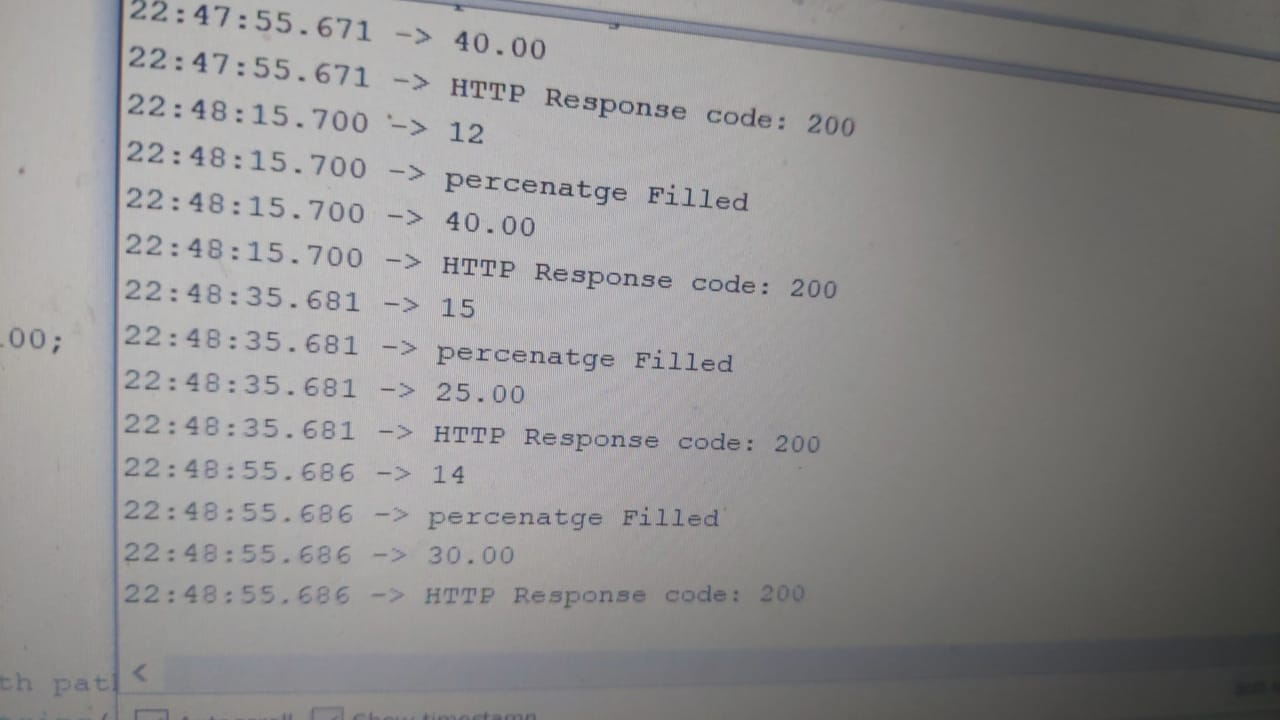
\includegraphics[scale=0.20]{check1.jpg}
    \caption{Fetching data from the sensor to the cloud}
\end{figure}
\begin{figure}[H]
\centering
    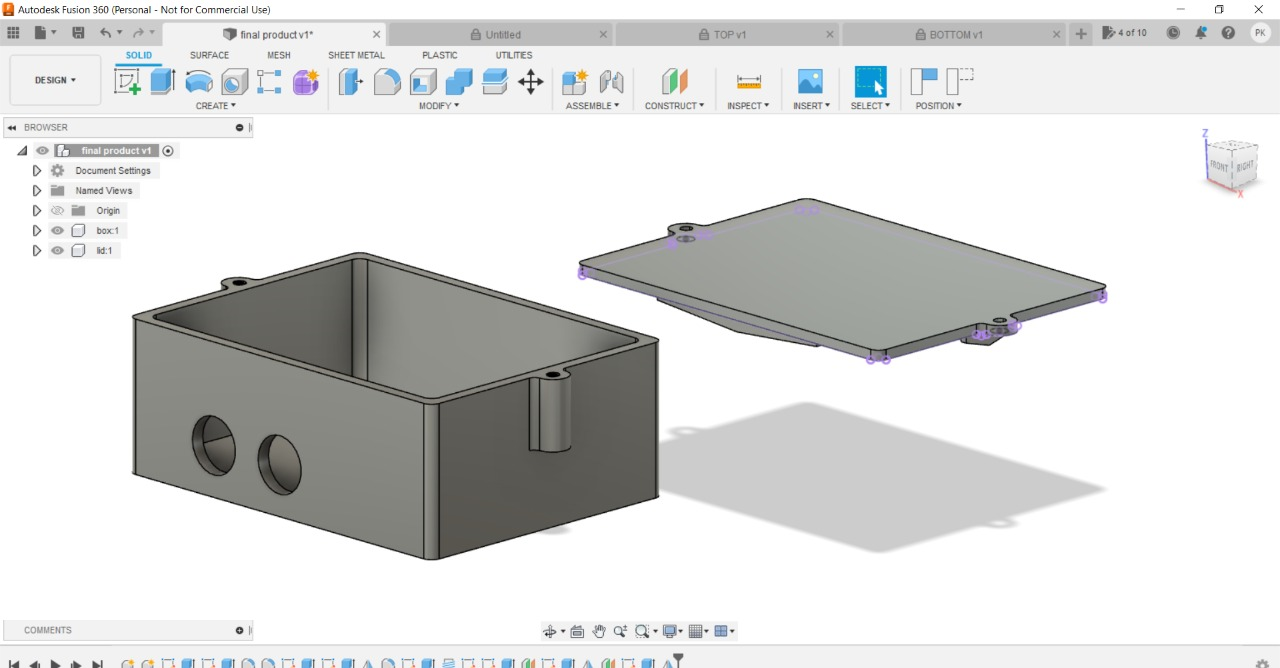
\includegraphics[scale=0.30]{3d_model1.jpg}
    \caption{3-D model of the case }
\end{figure}
\begin{figure}[H]
\centering
    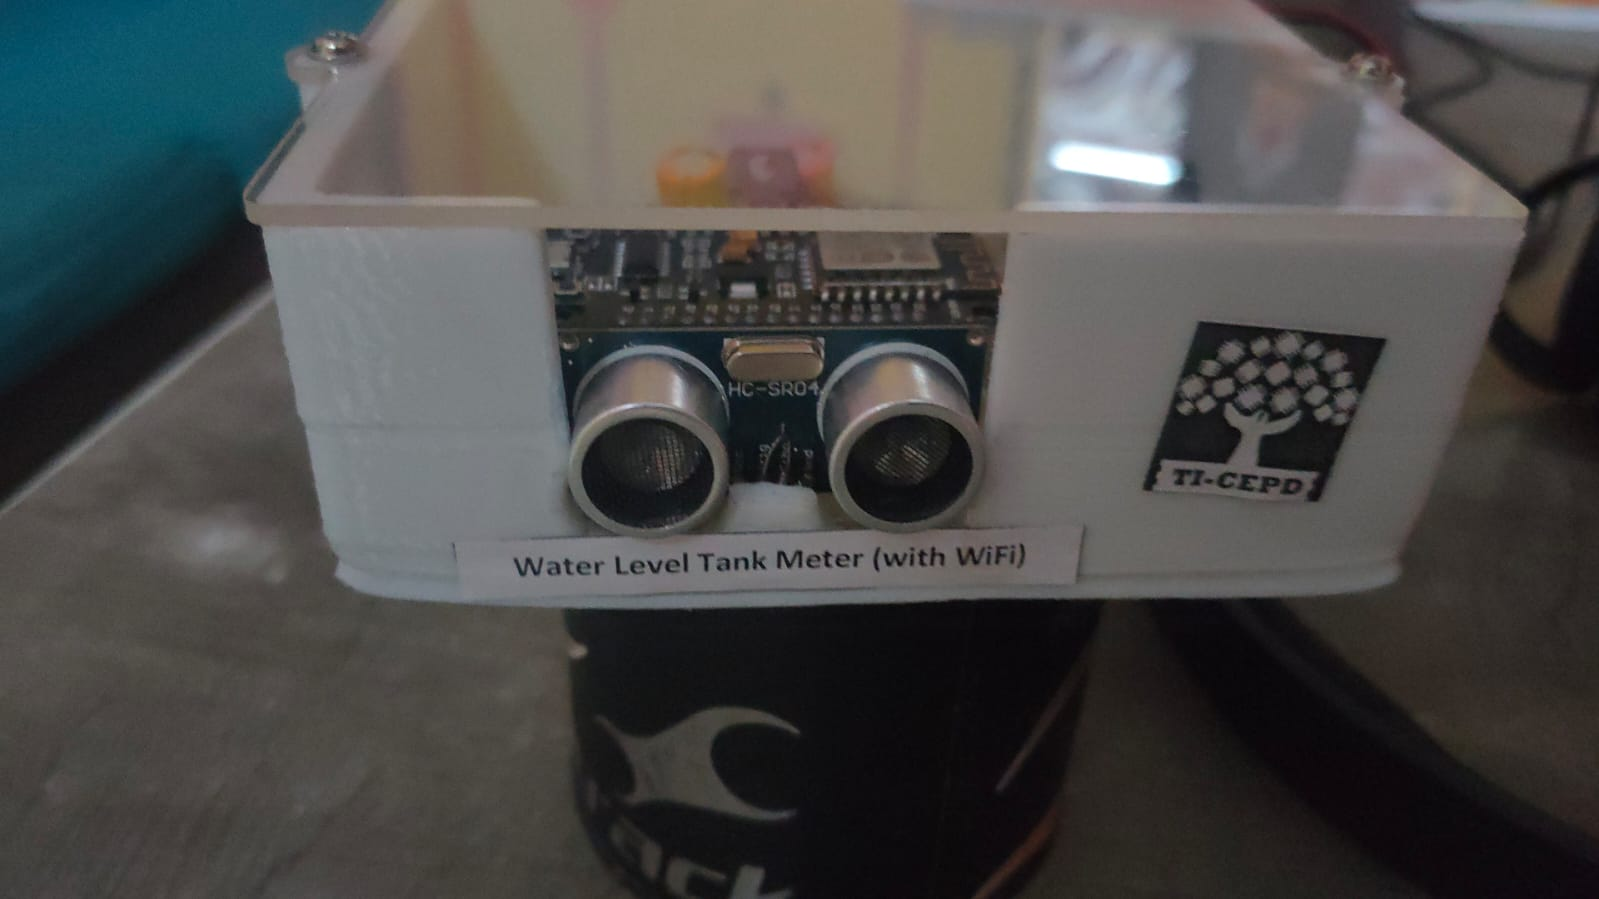
\includegraphics[scale=0.20]{final1.jpg}
    \caption{Final Assembled Project}
\end{figure}
\begin{figure}[H]
\centering
    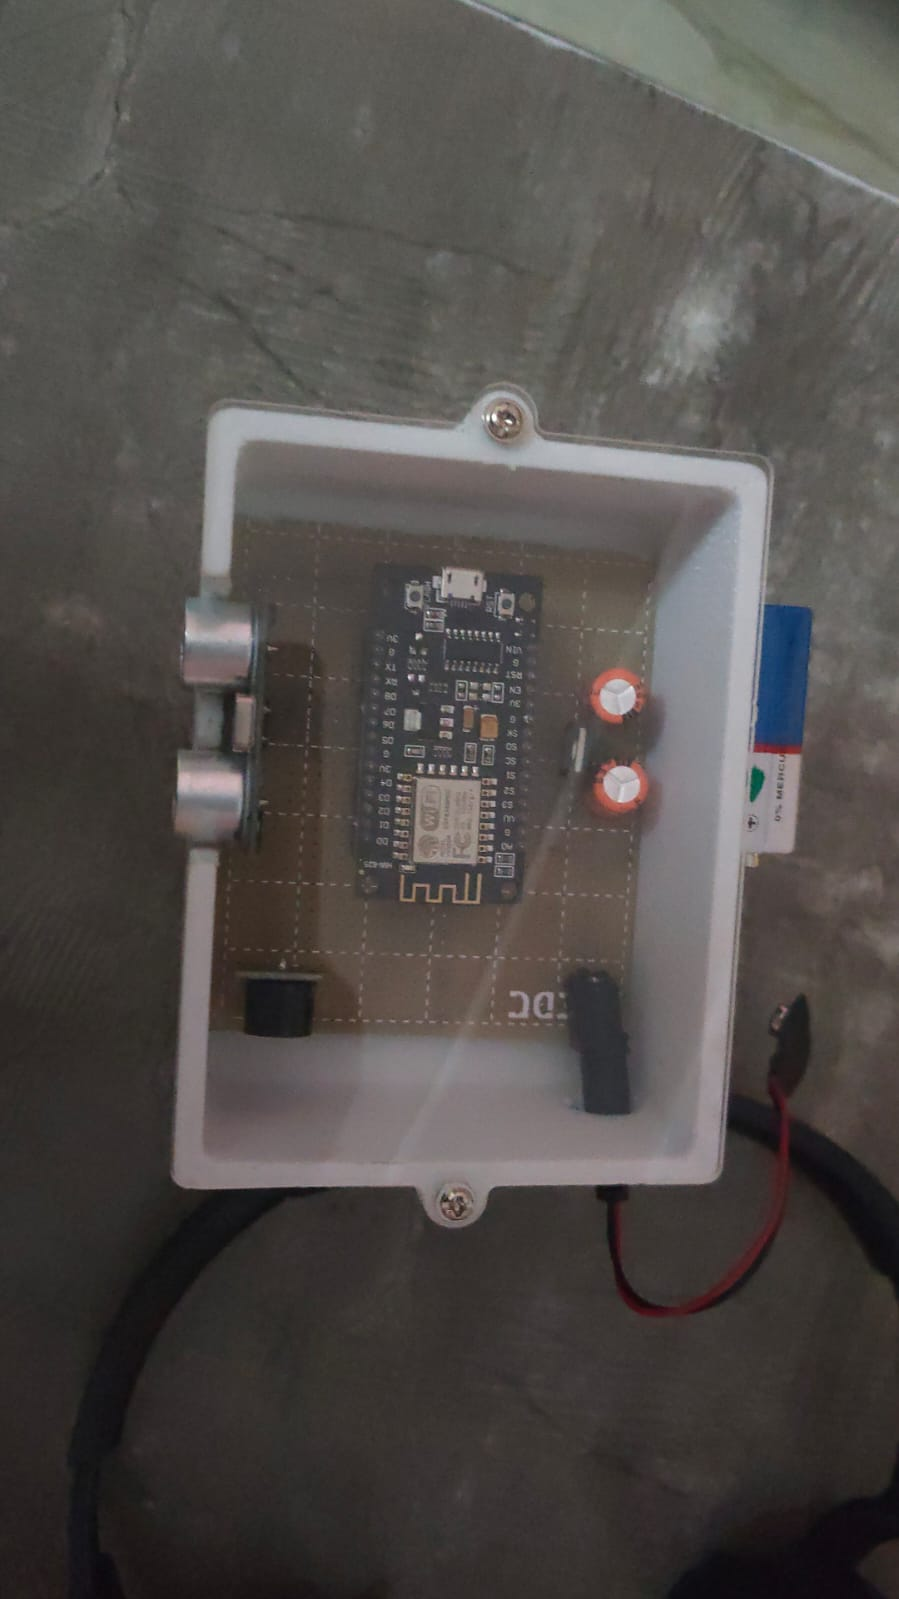
\includegraphics[scale=0.20]{final2.jpg}
    \caption{Final Assembled Project}
\end{figure}

\end{document}


